\documentclass{article}
%% 1. CÀI ĐẶT CƠ BẢN & LỚP VĂN BẢN
\usepackage[utf8]{inputenc}
% \usepackage[T5]{fontenc} % Bỏ dòng này vì đã có T1 bên dưới, tránh xung đột
\usepackage[T1]{fontenc}
\usepackage[table,xcdraw]{xcolor}
\usepackage{tikz}
\usepackage{tcolorbox}

%% 2. BỐ CỤC TRANG & CANH LỀ (ĐÃ SỬA THEO YÊU CẦU)
\usepackage[a4paper, top=3.5cm, bottom=3cm, left=3.5cm, right=2cm]{geometry}
% Đã BỎ tùy chọn "twoside" để lề trang không bị lệch


%% 3. NGÔN NGỮ, FONT CHỮ & ĐỊNH DẠNG ĐOẠN VĂN (ĐÃ SỬA THEO YÊU CẦU)
\usepackage[vietnamese]{babel}
\usepackage{mathptmx} % Font Times New Roman
\usepackage{indentfirst}
% --- CÀI ĐẶT FONT, GIÃN DÒNG, THỤT LỀ MỚI ---
\renewcommand{\normalsize}{\fontsize{13}{15.6}\selectfont}
\linespread{1.5} % Giãn dòng 1.5
\setlength{\parindent}{1cm} % Thụt đầu dòng 1cm
\setlength{\parskip}{10pt} % Khoảng cách giữa các đoạn là 10pt
\setlength{\emergencystretch}{2em}


%% 4. TÙY CHỈNH CÁC CẤP ĐỀ MỤC (SECTION, SUBSECTION,...)
\usepackage{titlesec}
\setcounter{secnumdepth}{4}

% Định dạng cho các chương CÓ ĐÁNH SỐ 
\titleformat{\section}[block]
  {\fontsize{16pt}{0pt}\selectfont \bfseries \centering}
  {CHƯƠNG \thesection:}
  {0.5em}
  {}
\titlespacing*{\section}{0pt}{0pt}{15pt}

% Định dạng cho các chương KHÔNG ĐÁNH SỐ
\titleformat{name=\section,numberless}[display]
  {\fontsize{16pt}{0pt}\selectfont \bfseries \centering}
  {}
  {0em}
  {}

% Định dạng cho các mục con
\titleformat*{\subsection}{\fontsize{14pt}{0pt}\selectfont \bfseries}
\titlespacing*{\subsection}{0pt}{3pt}{0pt}

\titleformat*{\subsubsection}{\fontsize{13pt}{0pt}\selectfont \bfseries \itshape}
\titlespacing*{\subsubsection}{0pt}{6pt}{0pt}

\titleformat*{\paragraph}{\fontsize{13pt}{0pt}\selectfont \itshape}
\titlespacing*{\paragraph}{0pt}{0pt}{0pt}

\titleformat{\paragraph}
  {\normalfont\fontsize{13pt}{0pt}\selectfont\itshape}
  {\theparagraph}
  {1em}
  {}
\titlespacing*{\paragraph}{0pt}{0.5ex plus 0.5ex minus .2ex}{0.5ex plus .2ex}


%% 5. HÌNH ẢNH, BẢNG BIỂU & CHÚ THÍCH (CAPTION)
\usepackage[nottoc]{tocbibind}
\usepackage{tocloft}
\setlength{\cftbeforesecskip}{6pt}
\setlength{\cftbeforesubsecskip}{2pt}
\setlength{\cftbeforesubsubsecskip}{1pt}

% Căn giữa các tiêu đề danh mục tương tự tiêu đề section gốc
\renewcommand{\cfttoctitlefont}{\hspace*{\fill}\fontsize{16pt}{0pt}\selectfont\bfseries}
\renewcommand{\cftaftertoctitle}{\hspace*{\fill}}
\renewcommand{\cftloftitlefont}{\hspace*{\fill}\fontsize{16pt}{0pt}\selectfont\bfseries}
\renewcommand{\cftafterloftitle}{\hspace*{\fill}}
\renewcommand{\cftlottitlefont}{\hspace*{\fill}\fontsize{16pt}{0pt}\selectfont\bfseries}
\renewcommand{\cftafterlottitle}{\hspace*{\fill}}
\usepackage{graphicx}
\usepackage{float}
\usepackage{longtable}
\usepackage{tabularx}
\usepackage{multirow}
\usepackage[font=normal]{caption}
\usepackage{array}

\renewcommand{\figurename}{\fontsize{12pt}{0pt}\selectfont Hình}
\captionsetup[figure]{labelsep=space}

\renewcommand{\tablename}{\fontsize{12pt}{0pt}\selectfont Bảng}
\captionsetup[table]{labelsep=space}

\newcolumntype{s}{>{\hsize=.3\hsize}X}
\newcolumntype{y}{>{\hsize=.4\hsize}X}
\newcolumntype{d}{>{\hsize=.1\hsize}X}
\newcolumntype{a}{>{\hsize=1.1\hsize}X}
\newcolumntype{g}{>{\hsize=5\hsize}X}
\newcolumntype{P}[1]{>{\raggedright\arraybackslash}p{#1}}
% --- SỬA LỖI TẠI ĐÂY ---
% \renewcommand{\tabularxcolumn}[1]{>{\small}m{#1}} % Dòng lệnh cũ gây lỗi thu nhỏ chữ
\renewcommand{\tabularxcolumn}[1]{>{\raggedright\arraybackslash}m{#1}} % Lệnh mới: Bỏ \small, thêm căn lề trái cho đẹp
% -----------------------


%% 6. KHỐI LỆNH (CODE LISTINGS) 
\usepackage{listings}
% Gói xcolor đã được nạp ở mục 5, không cần nạp lại

\lstdefinestyle{customcode}{
    basicstyle=\small\ttfamily,
    breaklines=true,
    numbers=left,
    numberstyle=\tiny\color{gray},
    keywordstyle=\color{blue!80!black}\bfseries,
    commentstyle=\color{green!50!black}\itshape,
    stringstyle=\color{red!70!black},
    showstringspaces=false,
    tabsize=2,
    captionpos=b,
    frame=single,
    rulecolor=\color{gray!40},
    xleftmargin=1.5em,
    framexleftmargin=1em,
    aboveskip=1.5em,
    belowskip=1.5em
}
\renewcommand{\lstlistingname}{Khối lệnh}


%% 7. TOÁN HỌC & CÁC MÔI TRƯỜNG ĐỊNH LÝ
\newtheorem{theorem}{Định lý}[section]
\newtheorem{defn}[theorem]{Định nghĩa}
\newtheorem{corollary}[theorem]{Hệ quả}
\newtheorem{lemma}[theorem]{Bổ đề}


%% 8. TÀI LIỆU THAM KHẢO
\usepackage[natbibapa]{apacite} 
\bibliographystyle{apacite}
\makeatletter
\def\APAC@apcfile{english.apc}
\makeatother

%% 9. CÁC GÓI BỔ SUNG KHÁC
\usepackage{wrapfig}
% Gói tikz đã được nạp ở mục 1, không cần nạp lại
\usetikzlibrary{calc,backgrounds}
\usepackage{soul}
\usepackage{colortbl}
\usepackage{forloop}
\usepackage{enumitem}

\definecolor{LightCyan}{rgb}{0.88,1,1}
\newcounter{loopcntr}
\newcommand{\rpt}[2][1]{\forloop{loopcntr}{0}{\value{loopcntr}<#1}{#2}}
\setitemize{itemsep=0pt,leftmargin=1.25cm,topsep = 3pt}


%% 10. ĐÁNH SỐ TỰ ĐỘNG & LIÊN KẾT 
\usepackage{chngcntr}
\usepackage[unicode, plainpages=false, pdfpagelabels=true, hidelinks]{hyperref}

% Cấu hình bộ đếm cho các môi trường
\counterwithin{figure}{section}
\counterwithin{table}{section}
\counterwithin{equation}{section}
% Các counter khác đã được article class và titlesec xử lý, không cần thêm


%% 11. ĐỊNH NGHĨA LẠI TÊN CÁC THÀNH PHẦN CỦA TÀI LIỆU
\AtBeginDocument{%
  \renewcommand{\contentsname}{MỤC LỤC}
  \renewcommand{\listfigurename}{DANH MỤC HÌNH VẼ}
  \renewcommand{\listtablename}{DANH MỤC BẢNG BIỂU}
  \renewcommand{\refname}{TÀI LIỆU THAM KHẢO}
  \normalsize % Áp dụng cỡ chữ mặc định cho toàn bộ tài liệu
}


%% 12. CÁC BIẾN TOÀN CỤC SỬ DỤNG TRONG BÁO CÁO
\newcommand{\khoa}{CÔNG NGHỆ THÔNG TIN}
\newcommand{\mon}{DỰ ÁN CÔNG NGHỆ THÔNG TIN}
\newcommand{\chuyennganh}{MẠNG MÁY TÍNH VÀ TRUYỀN THÔNG DỮ LIỆU}
\newcommand{\de}{XÂY DỰNG MẠNG CAMPUS NETWORK SỬ DỤNG SDN VÀ SD-WAN}
\newcommand{\gvhd}{ThS. LÊ VIẾT THANH}
\newcommand{\svmot}{TRẦN HỮU NHÂN - 52300235}
\newcommand{\svhai}{NGUYỄN NHẬT HÀO - 52300198}
\newcommand{\lop}{23050401}
\newcommand{\khoahoc}{27}
\newcommand{\nam}{2026}

\newcommand{\loaibaocao}{BÁO CÁO GIỮA KỲ}
\newcommand{\mocbaocao}{01/10/2026}
 % Dùng chung preamble với báo cáo chính

\begin{document}

	% --- PHẦN BÌA (KHÔNG ĐÁNH SỐ) ---
	\hypersetup{pageanchor=false}
	\pagenumbering{gobble}

	\pagenumbering{gobble}
\begin{center}
	\fontsize{14pt}{0pt}\selectfont TỔNG LIÊN ĐOÀN LAO ĐỘNG VIỆT NAM \\
	\fontsize{14pt}{0pt}\selectfont \textbf{TRƯỜNG ĐẠI HỌC TÔN ĐỨC THẮNG} \\
	\fontsize{14pt}{0pt}\selectfont \textbf{KHOA \khoa} \\\vspace*{6 pt}		
\includegraphics[width=0.3\linewidth]{image/logo-tdtu.jpg}\\\vspace*{0.3cm}

	\fontsize{14pt}{0pt}\selectfont \textbf{\svmot}\\\vspace{6pt}
    \fontsize{14pt}{0pt}\selectfont \textbf{\svhai}\\\vspace{11pt}
    \vspace*{2.5cm}
	\fontsize{24pt}{0pt}\selectfont 
    \textbf{\de}\\\vspace*{2cm}
    
	\fontsize{20pt}{0pt}\selectfont \textbf{\loaibaocao}\\\vspace*{10pt}
	\fontsize{18pt}{0pt}\selectfont \textbf{\mon}\\\vspace*{6pt}
        \fontsize{18pt}{0pt}\selectfont \textbf{\chuyennganh}\\\vspace*{2.5cm}
 
	\fontsize{14pt}{0pt}\selectfont \textbf{THÀNH PHỐ HỒ CHÍ MINH, \nam} \\
  
\end{center}
\newpage
      % Trang bìa 1
	\begin{center}
	\fontsize{14pt}{0pt}\selectfont TỔNG LIÊN ĐOÀN LAO ĐỘNG VIỆT NAM \\
	\fontsize{14pt}{0pt}\selectfont \textbf{TRƯỜNG ĐẠI HỌC TÔN ĐỨC THẮNG} \\
	\fontsize{14pt}{0pt}\selectfont \textbf{KHOA \khoa} \\\vspace*{6pt}	
    
\includegraphics[width=0.3\linewidth]{image/logo-tdtu.jpg}\\\vspace*{0.5cm}
 
	\fontsize{14pt}{0pt}\selectfont \textbf{\svmot}\\\vspace{6pt}
    \fontsize{14pt}{0pt}\selectfont \textbf{\svhai}\\\vspace{11pt}

    \vspace*{2cm}

	\fontsize{24pt}{0pt}\selectfont \textbf{\de}\\\vspace*{1.4cm}

	\fontsize{20pt}{0pt}\selectfont \textbf{\loaibaocao}\\\vspace*{10pt}
	\fontsize{18pt}{0pt}\selectfont \textbf{\mon}\\\vspace*{6pt}
        \fontsize{18pt}{0pt}\selectfont \textbf{\chuyennganh}\\\vspace*{1.2cm}
        
        \fontsize{14pt}{0pt}\selectfont Người hướng dẫn\\\vspace{6pt}
	\fontsize{14pt}{0pt}\selectfont \textbf{\gvhd} \\\vspace*{1.2cm}
 
	\fontsize{14pt}{0pt}\selectfont \textbf{THÀNH PHỐ HỒ CHÍ MINH, \nam} \\
  
\end{center}	
\newpage
   % Trang bìa 2

	% --- PHẦN ĐẦU CỦA BÁO CÁO ---
	\cleardoublepage
	\hypersetup{pageanchor=true}
	\pagenumbering{roman}
	\setcounter{page}{3}

	\section*{\fontsize{18pt}{18pt}\selectfont\MakeUppercase{\de}\\TÓM TẮT BÁO CÁO GIỮA KỲ}

Báo cáo giữa kỳ tổng hợp kết quả thực hiện đề tài ``Xây dựng mạng Campus Network sử dụng SDN và SD-WAN'' tính đến mốc \mocbaocao{}, tương ứng khoảng giữa kế hoạch tổng thể từ 08/08/2026 đến 21/11/2026. Mục đích của báo cáo là trình bày những gì nhóm đã thiết kế và triển khai được, mức độ kiểm chứng của từng hạng mục, các vấn đề kỹ thuật đã gặp cùng cách xử lý, và kế hoạch cho nửa còn lại của dự án.

Mô hình được xây dựng trên EVE-NG gồm Campus chính (Site 100), ba cơ sở phụ Cần Thơ, Đà Nẵng, Nha Trang (Site 200, 300, 400), vùng điều khiển SD-WAN (Site 900) và hai mạng truyền tải Internet/MPLS. Tại Campus chính, kiến trúc Core--Distribution--Access được kết hợp với SDN: bộ điều khiển Ryu quản lý sáu switch Open vSwitch bằng OpenFlow 1.3 qua VLAN quản trị 99. Liên kết giữa các cơ sở sử dụng Cisco SD-WAN (Viptela 20.10.1) với vManage, vSmart, vBond, tám vEdge và underlay eBGP.

Đến thời điểm giữa kỳ, nhóm đã hoàn thành giai đoạn khảo sát, thiết kế tổng thể và phần lớn giai đoạn triển khai: hạ tầng LAN Campus chính (VRRP, OSPF, firewall ASAv HA), DHCP tập trung, SDN với 6/6 OVS kết nối Ryu, fabric SD-WAN với 8/8 vEdge lên controller và 56/56 phiên BFD hoạt động, định tuyến liên site qua service VPN và các chính sách tập trung (SLA, Application-Aware Routing, data policy). Các hạng mục đang thực hiện gồm kiểm thử tích hợp có kịch bản failover, mở rộng chi nhánh mới theo mô hình mạng phẳng (Site 500) và hoàn thiện báo cáo cuối kỳ.

Báo cáo gồm năm chương: Chương 1 giới thiệu đề tài và kế hoạch; Chương 2 tóm tắt cơ sở lý thuyết; Chương 3 trình bày thiết kế hệ thống; Chương 4 báo cáo tiến độ và kết quả đạt được; Chương 5 nêu kế hoạch giai đoạn cuối và kết luận giữa kỳ.

Về phương pháp, nhóm triển khai theo từng lớp và chỉ chuyển sang lớp tiếp theo khi lớp bên dưới đã được kiểm chứng: hạ tầng vật lý và lớp 2, định tuyến nội bộ, firewall, dịch vụ DHCP, mặt phẳng điều khiển SDN, rồi mới tới fabric SD-WAN và chính sách. Toàn bộ cấu hình, file topology và nhật ký sự cố được lưu trong kho mã nguồn để có thể phục hồi lab và truy vết mọi thay đổi. Các kết quả nêu trong báo cáo đều đi kèm bằng chứng từ thiết bị (kết quả lệnh \texttt{show}, bảng flow, gói tin bắt được) thay vì chỉ dựa trên cấu hình.

Bên cạnh kết quả kỹ thuật, giai đoạn vừa qua giúp nhóm tích lũy kinh nghiệm vận hành thực tế: xử lý vòng lặp trên VLAN quản trị của SDN, cấp và ký chứng thư cho thiết bị SD-WAN, duy trì danh sách thiết bị được phép trên controller và chẩn đoán đường hầm BFD giữa các màu transport. Những kinh nghiệm này được tổng hợp thành quy trình phục hồi lab và sẽ là cơ sở cho các kịch bản kiểm thử dự phòng trong giai đoạn cuối.

\textbf{Từ khóa:} Campus Network, SDN, OpenFlow, Ryu, Open vSwitch, SD-WAN, Cisco Viptela, OMP, BFD, Application-Aware Routing, EVE-NG.

\newpage


	\tableofcontents
	\newpage

	\listoffigures
	\newpage

	\listoftables
	\newpage

	\newpage
\section*{DANH MỤC CÁC TỪ VIẾT TẮT}
\addcontentsline{toc}{section}{DANH MỤC CÁC TỪ VIẾT TẮT}

{
\renewcommand{\arraystretch}{1.3}
\begin{longtable}{ >{\centering\arraybackslash}p{3cm} p{9cm} }
    \textbf{Viết tắt} & \textbf{Tiếng Anh} \\

    AAR & Application-Aware Routing \\
    ACL & Access Control List \\
    API & Application Programming Interface \\
    AS & Autonomous System \\
    BFD & Bidirectional Forwarding Detection \\
    BGP & Border Gateway Protocol \\
    CA & Certificate Authority \\
    CLI & Command Line Interface \\
    CSR & Certificate Signing Request \\
    DHCP & Dynamic Host Configuration Protocol \\
    DMZ & Demilitarized Zone \\
    DNS & Domain Name System \\
    DPID & Datapath Identifier \\
    DTLS & Datagram Transport Layer Security \\
    HA & High Availability \\
    IOL & IOS on Linux \\
    LAN & Local Area Network \\
    MPLS & Multiprotocol Label Switching \\
    OMP & Overlay Management Protocol \\
    OSPF & Open Shortest Path First \\
    OVS & Open vSwitch \\
    PKI & Public Key Infrastructure \\
    SDN & Software-Defined Networking \\
    SD-WAN & Software-Defined Wide Area Network \\
    SLA & Service Level Agreement \\
    TLOC & Transport Locator \\
    VLAN & Virtual Local Area Network \\
    VPN & Virtual Private Network \\
    VRRP & Virtual Router Redundancy Protocol \\
    WAN & Wide Area Network \\
\end{longtable}
}


	% --- PHẦN THÂN CỦA BÁO CÁO ---
	\newpage
	\pagenumbering{arabic}

	\section{TỔNG QUAN ĐỀ TÀI}\label{sec:tong_quan}

\subsection{Lý do chọn đề tài}

Hạ tầng mạng của một trường đại học nhiều cơ sở phải phục vụ đồng thời đào tạo, nghiên cứu, hành chính và các dịch vụ số. Khi số khoa, phòng máy và cơ sở phụ tăng lên, mô hình cấu hình thủ công trên từng thiết bị bộc lộ hạn chế: thay đổi VLAN, thêm chi nhánh hay áp chính sách truy cập đều tốn thời gian và dễ sai sót. SDN tách mặt phẳng điều khiển khỏi thiết bị chuyển mạch để quản lý tập trung mạng nội bộ; SD-WAN cho phép kết nối nhiều cơ sở qua nhiều đường truyền và điều khiển đường đi theo chính sách. Kết hợp hai công nghệ này với kiến trúc Campus phân tầng là hướng tiếp cận phù hợp với nhu cầu thực tế của nhà trường.

\subsection{Mục tiêu đề tài}

\begin{itemize}
    \item Thiết kế mạng Campus đa cơ sở theo mô hình Core--Distribution--Access tại cơ sở chính và mô hình rút gọn tại các chi nhánh.
    \item Quy hoạch VLAN, địa chỉ IP, ASN và System-IP thống nhất, dễ mở rộng.
    \item Triển khai SDN với bộ điều khiển Ryu quản lý các switch Open vSwitch bằng OpenFlow 1.3.
    \item Triển khai SD-WAN Cisco (Viptela) kết nối các cơ sở qua hai mạng truyền tải Internet và MPLS, có chính sách chọn đường theo SLA.
    \item Xây dựng các kịch bản kiểm thử chức năng, dự phòng và đánh giá kết quả bằng bằng chứng thực nghiệm.
\end{itemize}

\subsection{Phạm vi và phương pháp thực hiện}

Toàn bộ hệ thống được mô phỏng trên một lab EVE-NG gồm 67 node và 100 network. Phạm vi gồm thiết kế logic, cấu hình thiết bị, dịch vụ mạng cơ bản (DHCP, DNS, Web, Mail, Syslog) và kiểm thử chức năng; không bao gồm triển khai trên phần cứng vật lý hay đo hiệu năng ở quy mô sản xuất.

Phương pháp thực hiện kết hợp nghiên cứu lý thuyết với triển khai và kiểm chứng trên lab. Mọi cấu hình được lưu trong kho mã nguồn (thư mục \texttt{configs/}, file topology \texttt{.unl}, tài liệu thiết kế) để truy vết. Khi xử lý sự cố, nhóm chẩn đoán theo lớp: vật lý/liên kết, lớp 2, lớp 3, dịch vụ, rồi mới tới ứng dụng, và chỉ kết luận khi có kết quả lệnh \texttt{show} hoặc gói tin bắt được làm bằng chứng.

\subsection{Yêu cầu đặt ra cho hệ thống}

Từ bối cảnh một trường đại học có một cơ sở chính và nhiều chi nhánh, nhóm xác định các yêu cầu chức năng mà mô hình cần đáp ứng:

\begin{itemize}
    \item Mỗi khoa, phòng ban thuộc một VLAN riêng; máy trạm nhận địa chỉ tự động qua DHCP và truy cập được các dịch vụ dùng chung (Web, Mail, DNS).
    \item Máy trạm tại các chi nhánh liên lạc được với Campus chính và với nhau thông qua mạng diện rộng, không phụ thuộc vào một nhà cung cấp đường truyền duy nhất.
    \item Switch tại Campus chính được quản lý tập trung từ bộ điều khiển SDN thay vì cấu hình riêng lẻ trên từng thiết bị.
    \item Lưu lượng giữa các site được điều khiển theo chính sách: chọn đường theo chất lượng, chặn các truy cập quản trị không được phép vào vùng máy chủ.
\end{itemize}

Bên cạnh đó là các yêu cầu phi chức năng:

\begin{itemize}
    \item \textbf{Tính sẵn sàng:} có dự phòng tại gateway, firewall và đường truyền WAN để một sự cố đơn lẻ không làm gián đoạn toàn bộ dịch vụ.
    \item \textbf{Bảo mật:} tách vùng người dùng, Server Farm và DMZ; thiết bị SD-WAN chỉ tham gia mạng khi được xác thực bằng chứng thư.
    \item \textbf{Khả năng mở rộng:} quy hoạch địa chỉ và định danh thống nhất để thêm chi nhánh mới mà không phải thiết kế lại.
    \item \textbf{Khả năng kiểm chứng:} mọi chức năng phải được chứng minh bằng kết quả thực tế trên lab.
\end{itemize}

\subsection{Kế hoạch tổng thể}

Dự án được chia thành sáu giai đoạn với 20 hạng mục công việc, tổng hợp trong Bảng~\ref{tab:ke_hoach_tong_the}. Mốc báo cáo giữa kỳ (\mocbaocao) nằm ở cuối giai đoạn triển khai và đầu giai đoạn kiểm thử tích hợp.

\begin{table}[H]
    \centering
    \small
    \caption{Các giai đoạn trong kế hoạch tổng thể}
    \label{tab:ke_hoach_tong_the}
    \begin{tabularx}{\textwidth}{|P{4.2cm}|c|P{2.6cm}|X|}
        \hline
        \textbf{Giai đoạn} & \textbf{Hạng mục} & \textbf{Thời gian} & \textbf{Đầu ra chính} \\
        \hline
        Khảo sát và lý thuyết & 1--3 & 06/2026--08/2026 & Phạm vi đề tài; lý thuyết SDN, SD-WAN \\
        \hline
        Thiết kế tổng thể & 4--6 & 07/2026--08/2026 & Kiến trúc 4 site; bảng IP/VLAN/ASN; topology EVE-NG \\
        \hline
        Triển khai hạ tầng Campus & 7--9 & 08/2026--09/2026 & Core/Dist/Access, firewall HA, DHCP \\
        \hline
        Triển khai SDN và SD-WAN & 10--16 & 08/2026--10/2026 & Ryu + 6 OVS; 3 controller + 8 vEdge; chi nhánh \\
        \hline
        Dịch vụ và kiểm thử tích hợp & 17--18 & 09/2026--11/2026 & Web/Mail/DNS/Syslog; kịch bản kiểm thử end-to-end \\
        \hline
        Báo cáo và bảo vệ & 19--20 & 11/2026 & Báo cáo cuối kỳ, slide, demo trên lab \\
        \hline
    \end{tabularx}
\end{table}

\subsection{Bố cục báo cáo giữa kỳ}

\begin{itemize}
    \item \textbf{Chương 1 -- Tổng quan đề tài:} lý do, mục tiêu, phạm vi, phương pháp và kế hoạch.
    \item \textbf{Chương 2 -- Cơ sở lý thuyết:} tóm tắt các công nghệ nền tảng được sử dụng.
    \item \textbf{Chương 3 -- Thiết kế hệ thống:} kiến trúc, topology, quy hoạch địa chỉ và các quyết định thiết kế.
    \item \textbf{Chương 4 -- Tiến độ và kết quả giữa kỳ:} các hạng mục đã hoàn thành, đang thực hiện, kết quả kiểm chứng và vấn đề đã xử lý.
    \item \textbf{Chương 5 -- Kế hoạch giai đoạn cuối và kết luận:} công việc còn lại, rủi ro và kết luận giữa kỳ.
\end{itemize}

	\newpage

	\section{CƠ SỞ LÝ THUYẾT}\label{sec:co_so_ly_thuyet}

Chương này tóm tắt các khái niệm nền tảng được sử dụng trong thiết kế. Nội dung chi tiết sẽ được trình bày đầy đủ trong báo cáo cuối kỳ.

\subsection{Mạng Campus phân tầng}

Mô hình Core--Distribution--Access chia mạng thành ba tầng có chức năng riêng: tầng Access kết nối thiết bị đầu cuối và gán VLAN; tầng Distribution tập trung lưu lượng, áp chính sách; tầng Core chuyển mạch tốc độ cao và định tuyến giữa các khối. Cách phân tầng giúp khoanh vùng sự cố, dễ mở rộng và tạo điều kiện bố trí dự phòng ở từng tầng (Hình~\ref{fig:core_distribution_access}).

\begin{figure}[H]
    \centering
    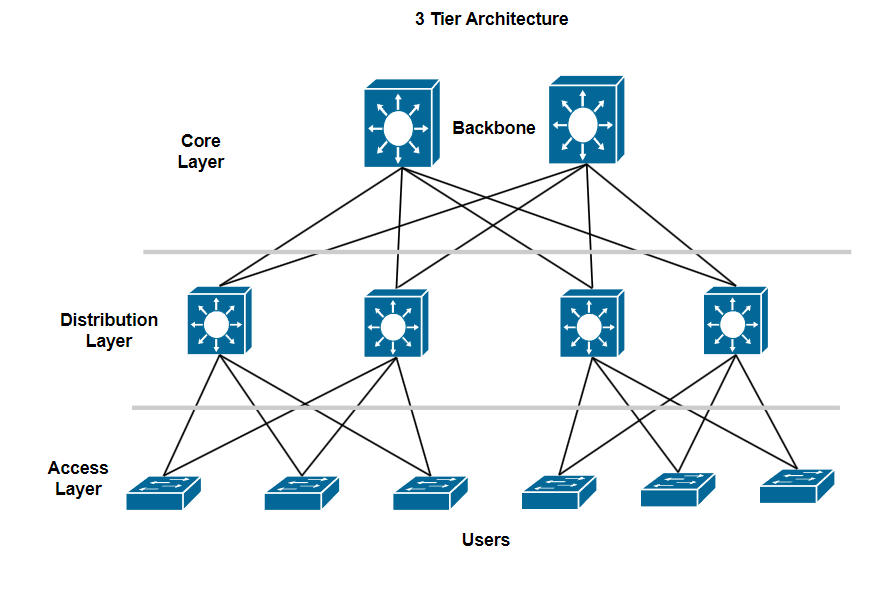
\includegraphics[width=0.70\textwidth]{image/mohinh.png}
    \caption{Mô hình mạng Campus Core--Distribution--Access}
    \label{fig:core_distribution_access}
\end{figure}

\subsection{VLAN, định tuyến và dự phòng gateway}

VLAN chia một hạ tầng lớp 2 thành nhiều miền quảng bá độc lập; các VLAN được mang trên đường trunk 802.1Q (Hình~\ref{fig:vlan}). Định tuyến liên VLAN thực hiện trên switch lớp 3 hoặc firewall. VRRP cho phép hai thiết bị chia sẻ một địa chỉ gateway ảo, để máy trạm không phải đổi gateway khi một thiết bị hỏng. OSPF được dùng để trao đổi tuyến nội bộ trong Campus chính, còn BGP được dùng giữa khách hàng và nhà cung cấp dịch vụ ở mạng truyền tải.

\begin{figure}[H]
    \centering
    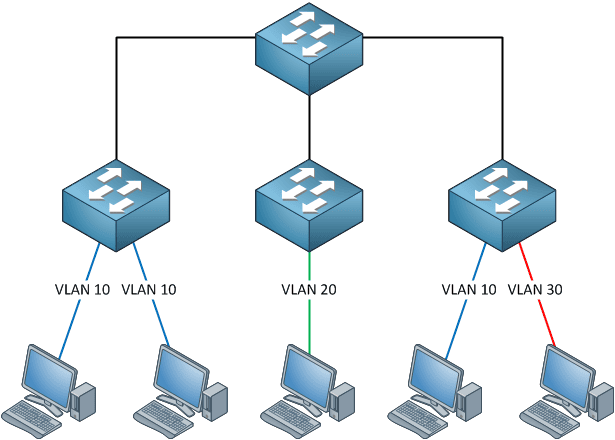
\includegraphics[width=0.65\textwidth]{image/vlan.png}
    \caption{Phân đoạn mạng bằng VLAN}
    \label{fig:vlan}
\end{figure}

\subsection{Software-Defined Networking}

SDN tách mặt phẳng điều khiển (control plane) khỏi mặt phẳng dữ liệu (data plane). Bộ điều khiển tập trung tính toán và cài đặt luật chuyển tiếp (flow) xuống switch qua giao thức southbound như OpenFlow; ứng dụng phía trên tương tác với bộ điều khiển qua API northbound (Hình~\ref{fig:sdn_architecture}).

\begin{figure}[H]
    \centering
    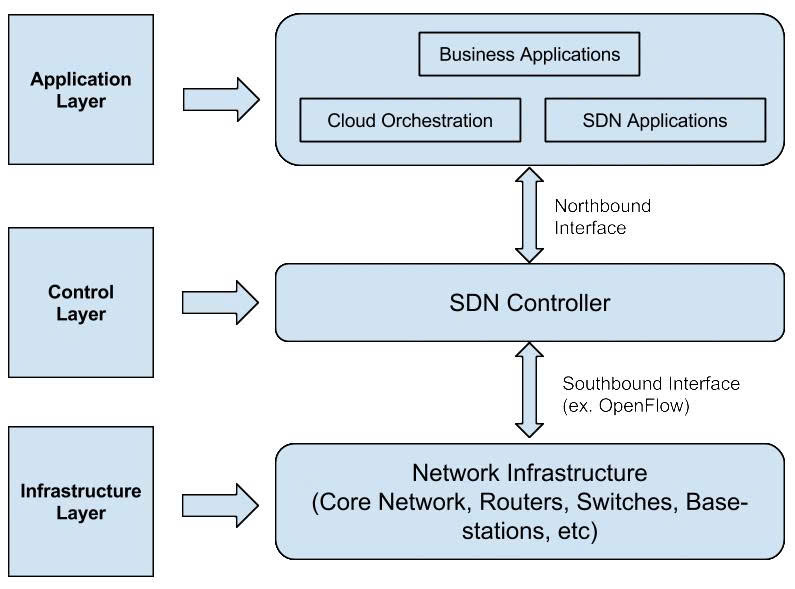
\includegraphics[width=0.55\textwidth]{image/SDN_ARCHITECTURE.jpg}
    \caption{Kiến trúc ba lớp của SDN}
    \label{fig:sdn_architecture}
\end{figure}

Trong OpenFlow 1.3, mỗi switch có các bảng flow gồm trường so khớp, độ ưu tiên và hành động. Gói tin không khớp flow nào sẽ rơi vào luật table-miss, thường được gửi lên bộ điều khiển dưới dạng \texttt{packet-in}. Bộ điều khiển học địa chỉ MAC, quyết định cổng ra và cài flow để các gói sau được chuyển trực tiếp trên switch (Hình~\ref{fig:sdn_hoat_dong}). Đề tài dùng bộ điều khiển Ryu (Python) và Open vSwitch làm switch OpenFlow.

\begin{figure}[H]
    \centering
    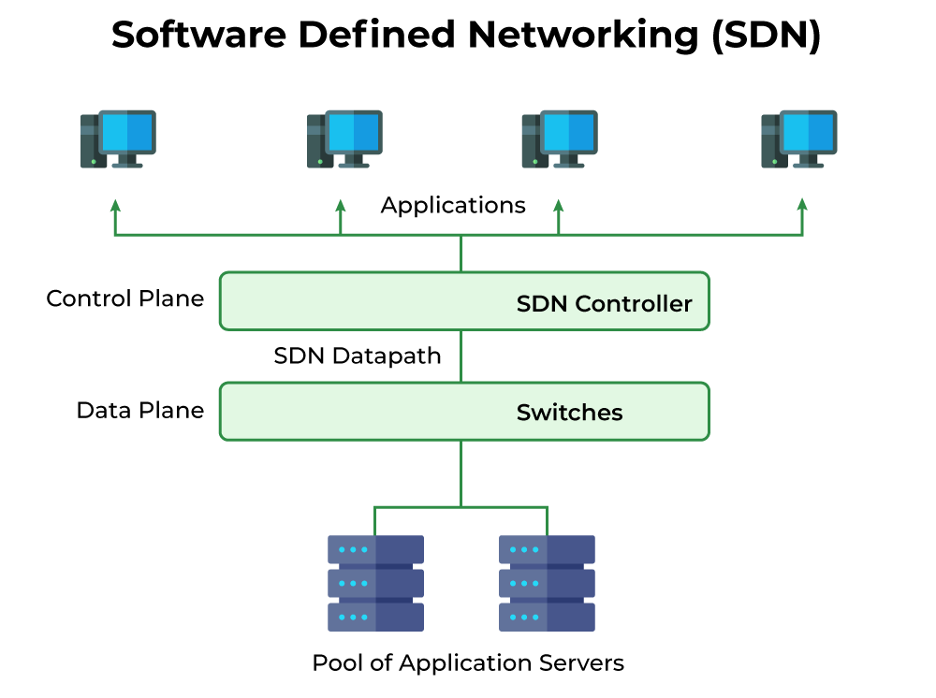
\includegraphics[width=0.70\textwidth]{image/nguyenlyhoatdongsdn.png}
    \caption{Nguyên lý hoạt động của SDN với OpenFlow}
    \label{fig:sdn_hoat_dong}
\end{figure}

\subsection{Software-Defined WAN (Cisco SD-WAN)}

Cisco SD-WAN (Viptela) gồm bốn thành phần (Hình~\ref{fig:sdwan}):

\begin{itemize}
    \item \textbf{vBond (orchestrator):} xác thực thiết bị và điều phối kết nối ban đầu.
    \item \textbf{vManage:} quản lý, cấu hình và giám sát tập trung.
    \item \textbf{vSmart:} bộ điều khiển định tuyến và chính sách, trao đổi tuyến với các edge qua OMP.
    \item \textbf{vEdge:} thiết bị tại site, thiết lập đường hầm IPsec tới các edge khác.
\end{itemize}

\begin{figure}[H]
    \centering
    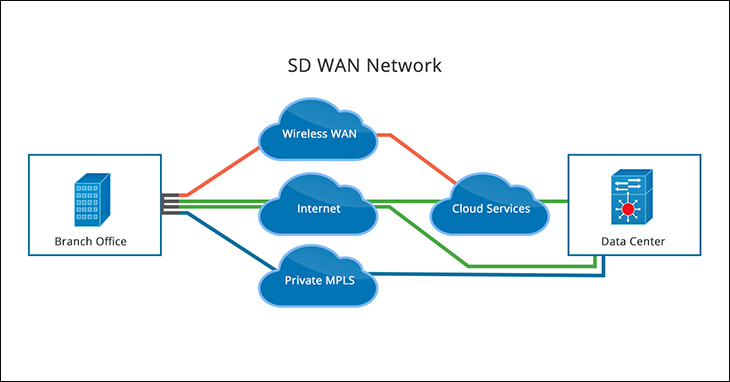
\includegraphics[width=0.70\textwidth]{image/sdwan.jpg}
    \caption{Kiến trúc Cisco SD-WAN}
    \label{fig:sdwan}
\end{figure}

Mỗi điểm kết nối WAN của vEdge là một TLOC, được gắn màu theo loại đường truyền (ví dụ \texttt{biz-internet}, \texttt{mpls}). BFD chạy trong từng đường hầm để phát hiện mất kết nối và đo độ trễ, jitter, tỷ lệ mất gói. Dựa trên số đo này, chính sách Application-Aware Routing chọn đường hầm đáp ứng SLA cho từng loại lưu lượng. Thiết bị chỉ tham gia fabric khi có chứng thư hợp lệ do CA tin cậy ký và có tên trong danh sách thiết bị được phép (whitelist) trên các controller.

\subsection{So sánh mạng truyền thống, SDN và SD-WAN}

SDN và SD-WAN cùng dựa trên nguyên lý tách mặt phẳng điều khiển và điều khiển tập trung, nhưng giải quyết hai bài toán khác nhau: SDN tập trung vào mạng nội bộ, còn SD-WAN tập trung vào kết nối giữa các cơ sở. Bảng~\ref{tab:so_sanh} tóm tắt sự khác biệt giữa ba cách tiếp cận.

\begin{table}[H]
    \centering
    \small
    \caption{So sánh mạng truyền thống, SDN và SD-WAN}
    \label{tab:so_sanh}
    \begin{tabularx}{\textwidth}{|P{2.6cm}|X|X|X|}
        \hline
        \textbf{Tiêu chí} & \textbf{Mạng truyền thống} & \textbf{SDN} & \textbf{SD-WAN} \\
        \hline
        Mặt phẳng điều khiển & Phân tán trên từng thiết bị & Tập trung tại controller & Tập trung tại vSmart \\
        \hline
        Phạm vi áp dụng & LAN và WAN & Chủ yếu LAN, data center & Kết nối WAN giữa các site \\
        \hline
        Cấu hình & Thủ công qua CLI từng thiết bị & Lập trình qua controller & Template, chính sách tập trung trên vManage \\
        \hline
        Giao thức chính & STP, OSPF, BGP & OpenFlow & OMP, BFD, IPsec \\
        \hline
        Chọn đường & Theo metric định tuyến & Theo flow do controller cài & Theo SLA ứng dụng (AAR) \\
        \hline
        Đường truyền & Thường phụ thuộc một nhà cung cấp & Không áp dụng & Nhiều transport (Internet, MPLS, LTE) \\
        \hline
    \end{tabularx}
\end{table}

Trong đề tài, hai công nghệ được kết hợp: SDN quản lý lớp Distribution--Access tại Campus chính, SD-WAN đảm nhận kết nối giữa Campus chính và các chi nhánh, còn firewall và Core vẫn dùng định tuyến truyền thống để làm điểm ghép nối giữa hai miền.

	\newpage

	\section{THIẾT KẾ HỆ THỐNG}\label{sec:thiet_ke}

\subsection{Kiến trúc tổng thể}

Hệ thống gồm năm vùng: Campus chính (Site 100), ba cơ sở phụ (Site 200 Cần Thơ, Site 300 Đà Nẵng, Site 400 Nha Trang), vùng điều khiển SD-WAN (Site 900) và hai mạng truyền tải độc lập là Internet (AS 64511) và MPLS (AS 64512). Từ tháng 10/2026, nhóm bổ sung Site 500 làm chi nhánh mới theo mô hình mạng phẳng để minh họa khả năng mở rộng. Topology logic được trình bày trong Hình~\ref{fig:topology_logic}.

\begin{figure}[H]
    \centering
    \resizebox{\textwidth}{!}{%
    \begin{tikzpicture}[
        font=\scriptsize,
        >=stealth,
        controller/.style={draw=purple!70!black, fill=purple!7, rounded corners, align=center, minimum height=1.2cm, text width=8.0cm},
        transport/.style={draw=black!70, fill=gray!12, rounded corners, align=center, minimum height=0.9cm, text width=3.5cm},
        campus/.style={draw=blue!65!black, fill=blue!5, rounded corners, align=center, minimum height=1.75cm, text width=6.2cm},
        branch/.style={draw=teal!70!black, fill=teal!5, rounded corners, align=center, minimum height=1.55cm, text width=4.4cm},
        newsite/.style={draw=orange!80!black, fill=orange!6, dashed, rounded corners, align=center, minimum height=1.55cm, text width=4.4cm},
        controlLink/.style={draw=purple!75!black, dashed, ->, line width=0.7pt},
        internetLink/.style={draw=blue!75!black, line width=0.9pt},
        mplsLink/.style={draw=orange!85!black, line width=0.9pt}
    ]
        \node[controller] (s900) at (0,3.7) {\textbf{Site 900 -- Control plane SD-WAN}\\
        vManage \texttt{10.9.0.10}; vSmart \texttt{10.9.0.11} (System-IP \texttt{10.9.0.13}); vBond \texttt{10.9.0.12}};

        \node[transport] (internet) at (-7.2,1.35) {\textbf{Internet underlay}\\AS 64511 -- color \texttt{biz-internet}};
        \node[transport] (mpls) at (7.2,1.35) {\textbf{MPLS underlay}\\AS 64512 -- color \texttt{mpls}};

        \node[campus] (s100) at (0,1.35) {\textbf{Site 100 -- Campus chính, AS 65000}\\
        vEdge1/2: \texttt{10.200.100.1/.2}, mỗi edge có Internet và MPLS\\
        ASAv HA -- Core-SW1/2 -- Ryu \texttt{10.1.99.10} điều khiển 6 OVS};

        \node[branch] (s200) at (-7.2,-2.1) {\textbf{Site 200 -- Cần Thơ, AS 65010}\\
        vEdge1 (MPLS), vEdge2 (Internet)\\Brand-FW -- VLAN 60/70};
        \node[branch] (s300) at (-2.4,-2.1) {\textbf{Site 300 -- Đà Nẵng, AS 65020}\\
        vEdge1 (MPLS), vEdge2 (Internet)\\Brand-FW -- VLAN 80/90};
        \node[branch] (s400) at (2.4,-2.1) {\textbf{Site 400 -- Nha Trang, AS 65030}\\
        vEdge1 (MPLS), vEdge2 (Internet)\\Brand-FW -- VLAN 50/60};
        \node[newsite] (s500) at (7.2,-2.1) {\textbf{Site 500 -- chi nhánh mới, AS 65040}\\
        1 vEdge (Internet + MPLS)\\Mạng phẳng \texttt{10.5.1.0/24}};

        \begin{pgfonlayer}{background}
            \draw[internetLink] (internet.east) -- (s100.west);
            \draw[mplsLink] (mpls.west) -- (s100.east);
            \foreach \b in {s200,s300,s400,s500} {
                \draw[internetLink] (internet.south) -- ([xshift=-6mm]\b.north);
                \draw[mplsLink] (mpls.south) -- ([xshift=6mm]\b.north);
            }
            \draw[controlLink] (s900.south) -- (s100.north);
        \end{pgfonlayer}

        \draw[internetLink] (-6.5,-3.5) -- (-5.5,-3.5) node[right, font=\scriptsize] {Internet};
        \draw[mplsLink] (-3.6,-3.5) -- (-2.6,-3.5) node[right, font=\scriptsize] {MPLS};
        \draw[controlLink] (-1.0,-3.5) -- (0.0,-3.5) node[right, font=\scriptsize] {control connection (mọi edge đều có, chỉ vẽ đại diện)};
        \node[font=\scriptsize] at (0,-3.95) {Khung nét đứt: site đang triển khai};
    \end{tikzpicture}%
    }
    \caption{Topology logic của hệ thống tại thời điểm giữa kỳ}
    \label{fig:topology_logic}
\end{figure}

Topology vật lý triển khai trên EVE-NG, gồm đầy đủ thiết bị, cổng kết nối và địa chỉ của từng site, được thể hiện trong Hình~\ref{fig:topology_eve}.

\begin{figure}[!htbp]
    \centering
    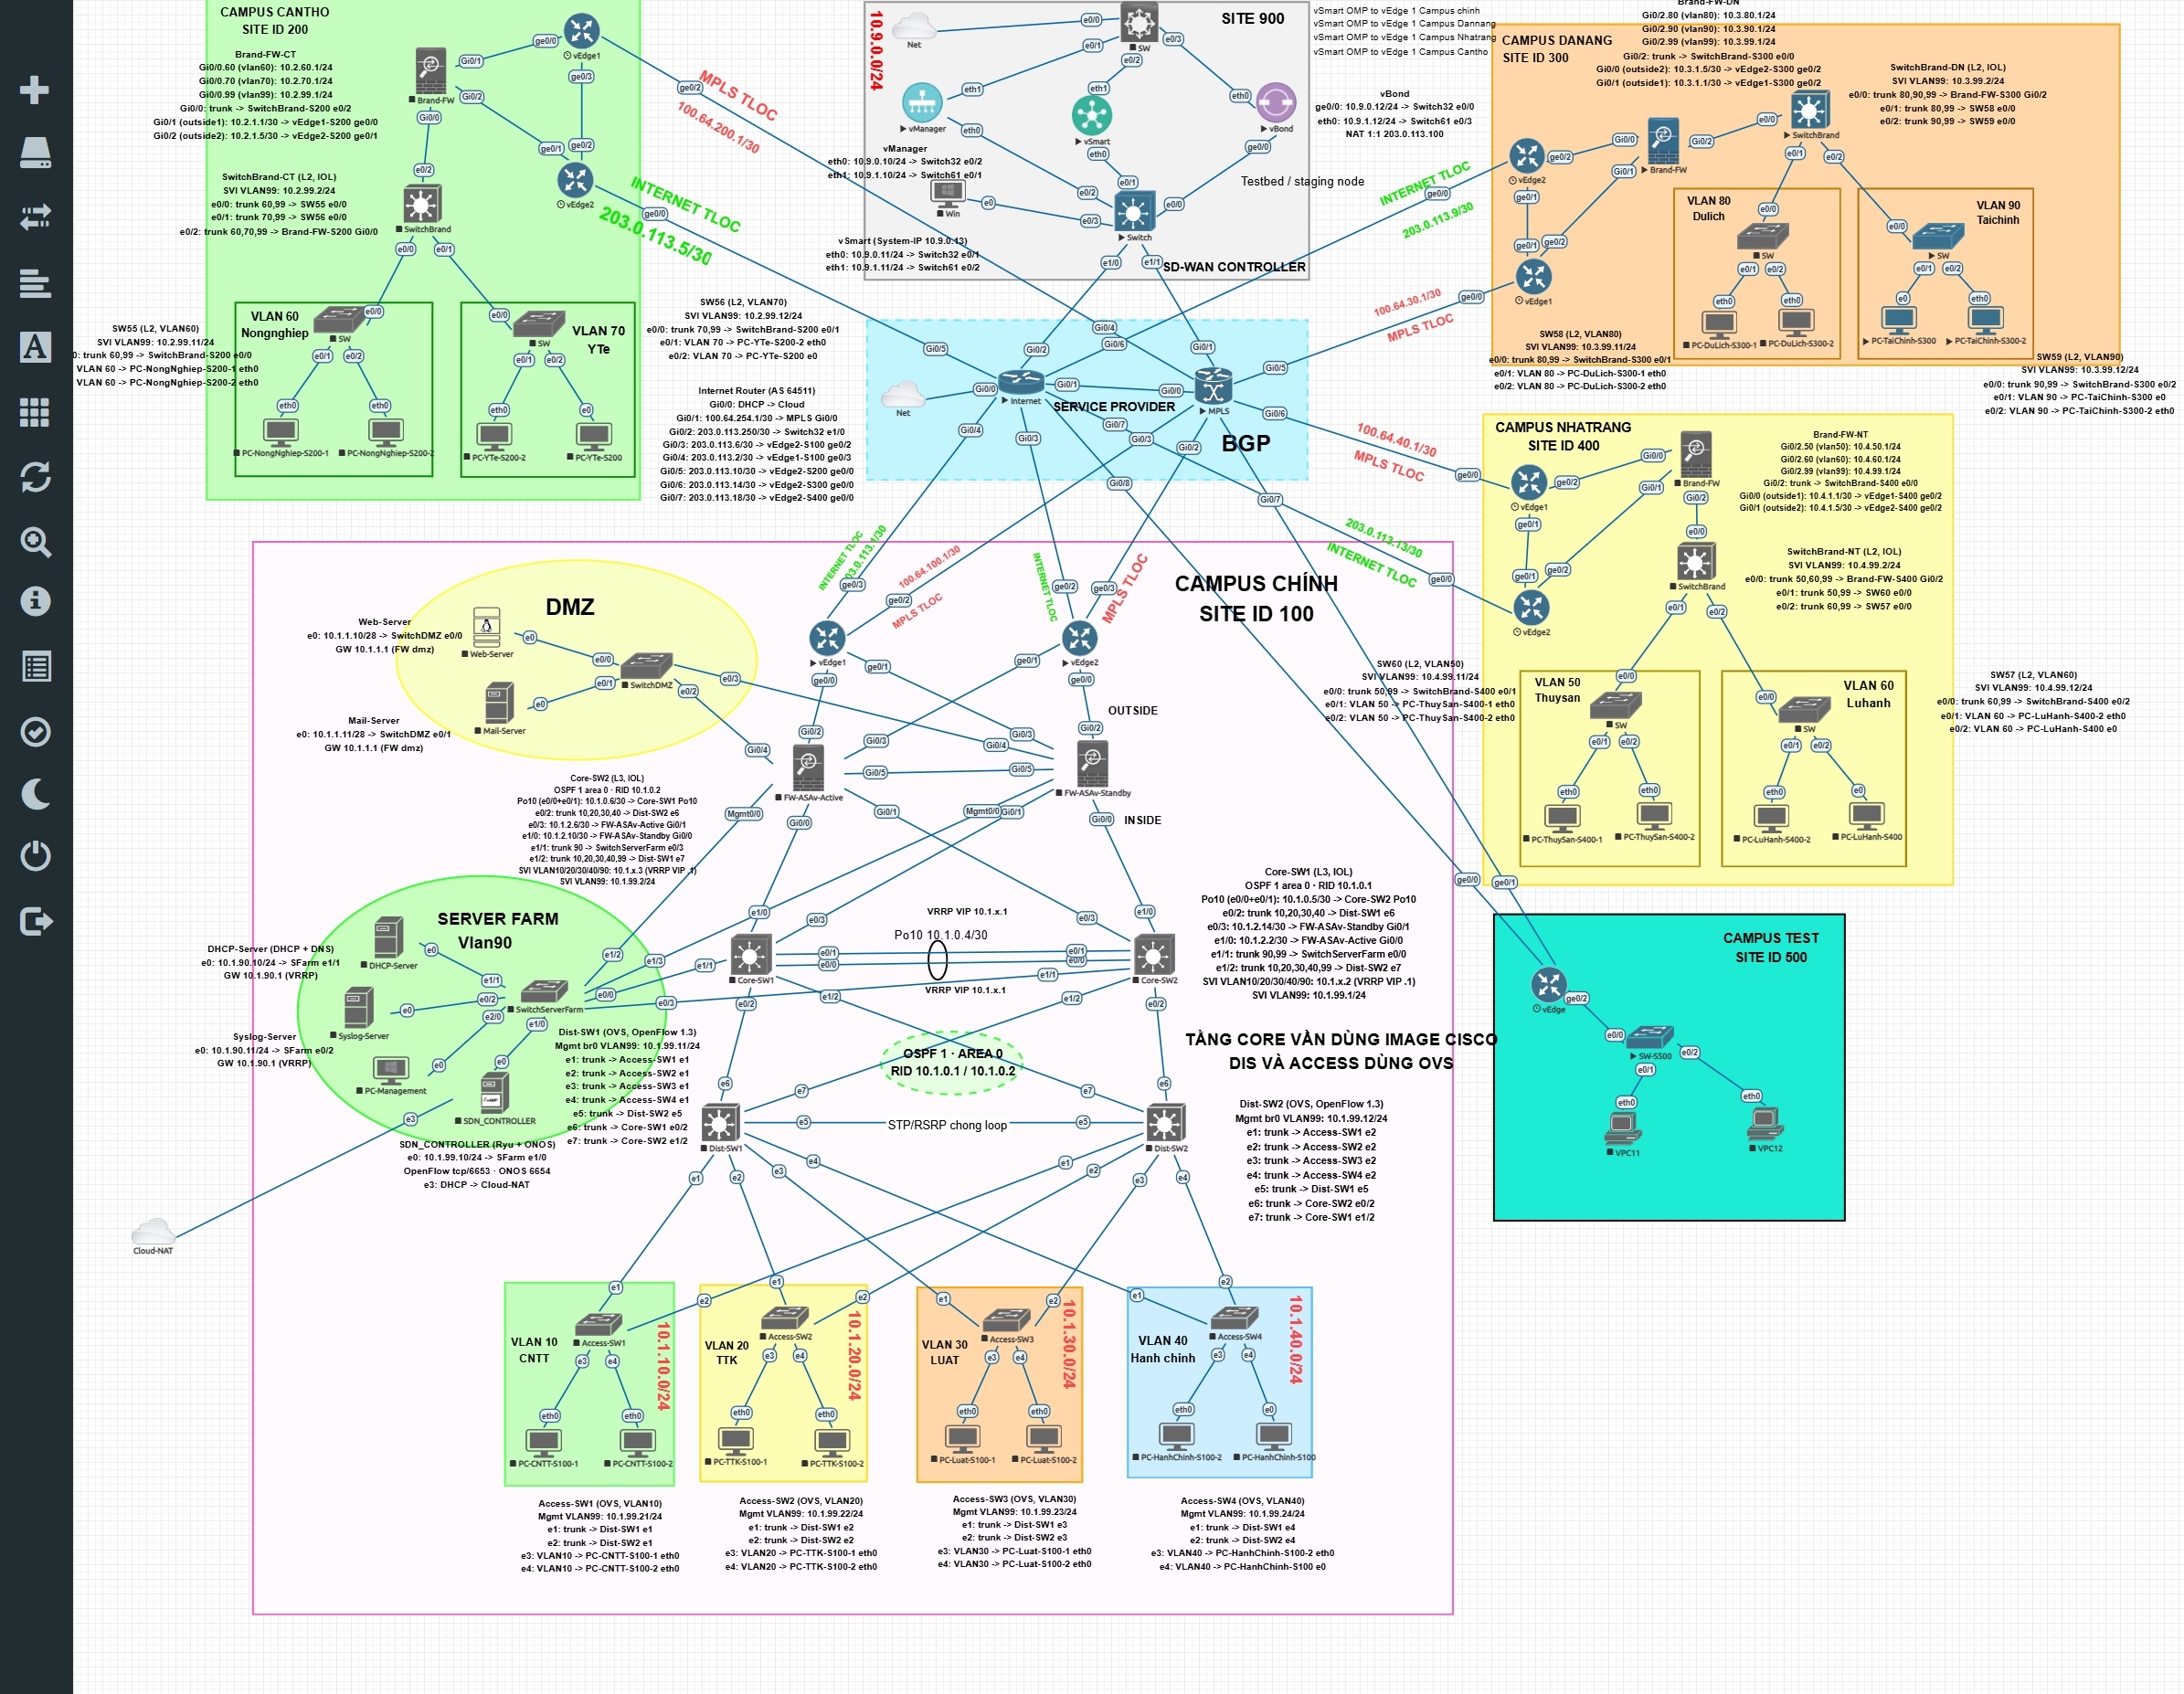
\includegraphics[width=1.0\textwidth]{image/topology.png}
    \caption{Topology vật lý tổng thể của hệ thống trên EVE-NG}
    \label{fig:topology_eve}
\end{figure}

\subsubsection{Campus chính (Site 100)}

Campus chính dùng mô hình ba tầng. Tầng Core gồm Core-SW1/2 (IOL), cung cấp gateway VRRP cho các VLAN và chạy OSPF Area 0 với firewall. Tầng Distribution (Dist-SW1/2) và Access (Access-SW1--4) là sáu Open vSwitch do Ryu điều khiển. Biên mạng là cặp firewall ASAv hoạt động active--standby, nối ra hai vEdge; mỗi vEdge có kết nối tới cả Internet và MPLS. Vùng Server Farm chứa DHCP Server, Syslog Server và SDN Controller; vùng DMZ chứa Web Server và Mail Server. Sơ đồ chi tiết Campus chính được trình bày trong Hình~\ref{fig:campus_chinh}.

\begin{figure}[!htbp]
    \centering
    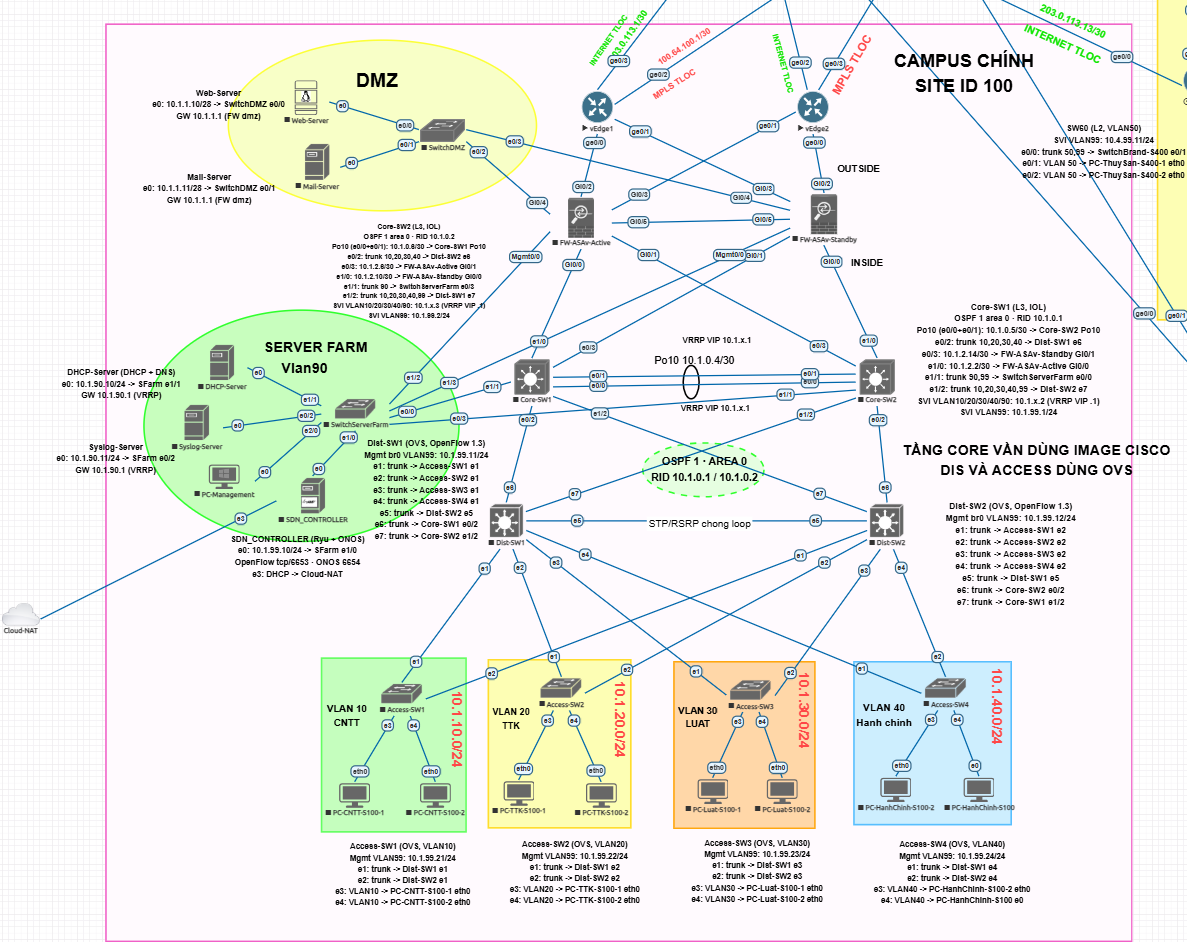
\includegraphics[width=1.0\textwidth]{image/campuschinh.png}
    \caption{Sơ đồ chi tiết Campus chính (Site 100) trên EVE-NG}
    \label{fig:campus_chinh}
\end{figure}


\subsubsection{Các cơ sở phụ (Site 200, 300, 400)}

Ba chi nhánh dùng chung khuôn \textit{Firewall-as-Core}: Brand-FW (ASAv) làm gateway cho các VLAN nghiệp vụ bằng sub-interface và cấp DHCP tại chỗ; SwitchBrand và hai switch phòng ban chỉ làm lớp 2. Mỗi chi nhánh có hai vEdge chia theo transport: vEdge1 nối MPLS, vEdge2 nối Internet. Sơ đồ triển khai của từng chi nhánh được trình bày trong các Hình~\ref{fig:site200}, \ref{fig:site300} và \ref{fig:site400}.

\begin{figure}[!htbp]
    \centering
    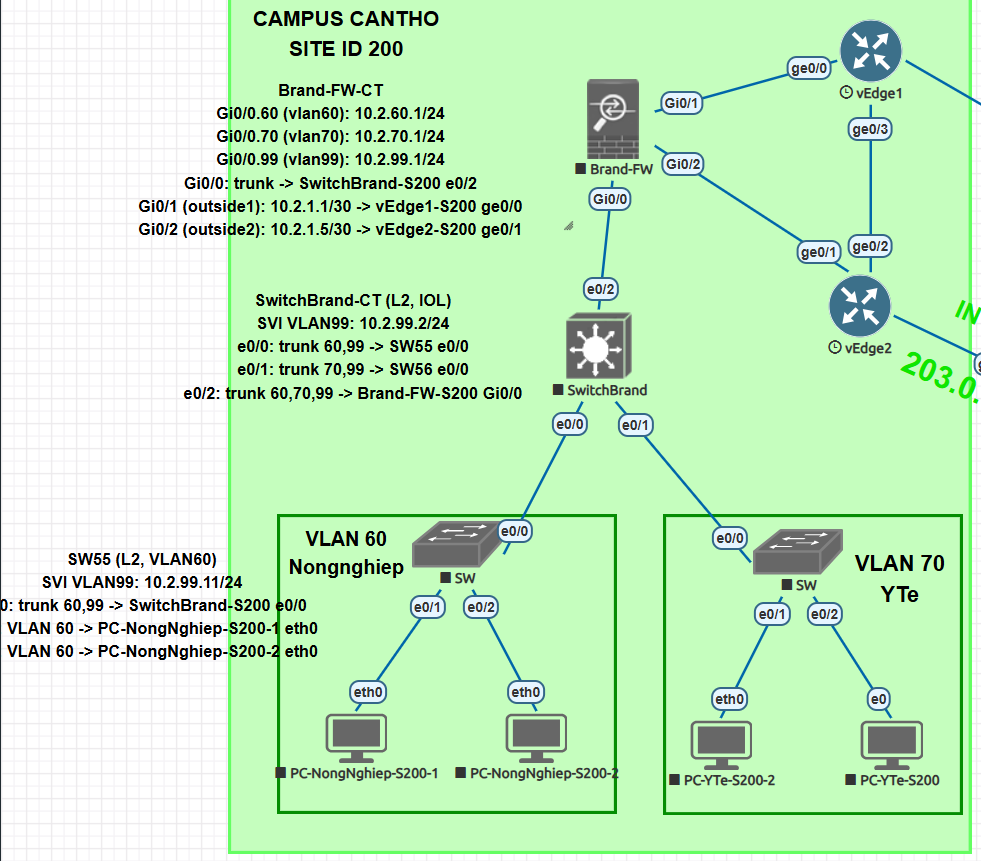
\includegraphics[width=0.75\textwidth]{image/site200.png}
    \caption{Sơ đồ chi nhánh Cần Thơ (Site 200)}
    \label{fig:site200}
\end{figure}

\begin{figure}[!htbp]
    \centering
    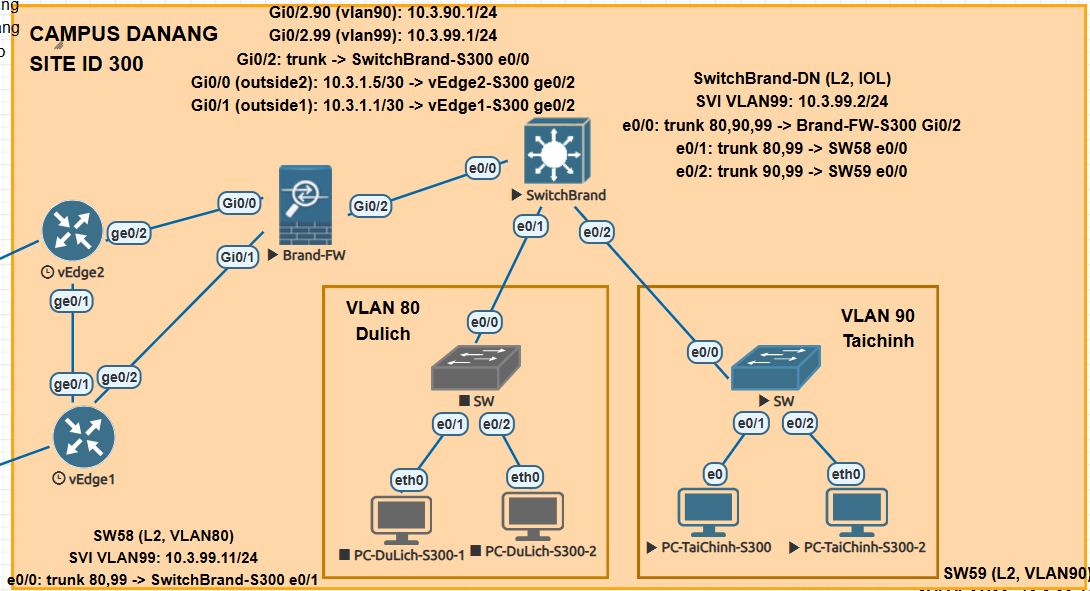
\includegraphics[width=0.80\textwidth]{image/site300.png}
    \caption{Sơ đồ chi nhánh Đà Nẵng (Site 300)}
    \label{fig:site300}
\end{figure}

\begin{figure}[!htbp]
    \centering
    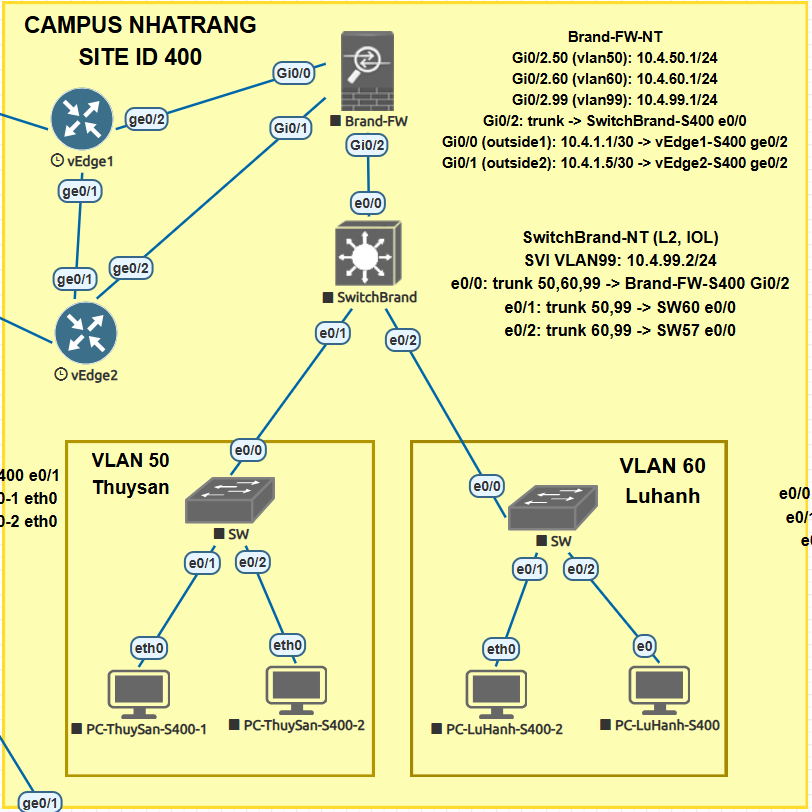
\includegraphics[width=0.80\textwidth]{image/site400.png}
    \caption{Sơ đồ chi nhánh Nha Trang (Site 400)}
    \label{fig:site400}
\end{figure}


\subsubsection{Chi nhánh mạng phẳng (Site 500)}

Site 500 được thiết kế cho cơ sở nhỏ: một vEdge vừa là router WAN, vừa là gateway và DHCP Server cho một subnet duy nhất \texttt{10.5.1.0/24}, không có firewall riêng và không chia VLAN. vEdge này có cả hai transport Internet và MPLS nên vẫn có dự phòng đường truyền, chỉ không có dự phòng thiết bị.

\subsection{Quy hoạch địa chỉ}

Toàn bộ mạng nội bộ dùng dải \texttt{10.0.0.0/8}, trong đó octet thứ hai biểu thị site: 1 (Campus chính), 2, 3, 4, 5 (các chi nhánh) và 9 (controller). Mỗi VLAN dùng subnet /24, gateway là địa chỉ \texttt{.1}, máy chủ dùng \texttt{.10/.11}, dải DHCP cho máy trạm là \texttt{.100--.199}. Liên kết điểm--điểm dùng /30.

\begin{table}[H]
    \centering
    \small
    \caption{Phân hoạch VLAN tại Campus chính}
    \label{tab:vlan_campus}
    \begin{tabularx}{\textwidth}{|c|P{3.2cm}|P{2.8cm}|X|}
        \hline
        \textbf{VLAN} & \textbf{Khu vực} & \textbf{Subnet} & \textbf{Ghi chú} \\
        \hline
        10 & Khoa Công nghệ thông tin & 10.1.10.0/24 & DHCP .100--.199, gateway VRRP .1 \\
        \hline
        20 & Khoa Toán -- Thống kê & 10.1.20.0/24 & DHCP .100--.199, gateway VRRP .1 \\
        \hline
        30 & Khoa Luật & 10.1.30.0/24 & DHCP .100--.199, gateway VRRP .1 \\
        \hline
        40 & Phòng Hành chính & 10.1.40.0/24 & DHCP .100--.199, gateway VRRP .1 \\
        \hline
        90 & Server Farm & 10.1.90.0/24 & DHCP Server .10, Syslog .11 \\
        \hline
        99 & Management và SDN & 10.1.99.0/24 & Controller .10, Dist .11/.12, Access .21--.24 \\
        \hline
        -- & DMZ & 10.1.1.0/28 & Web .10, Mail .11 \\
        \hline
    \end{tabularx}
\end{table}

\begin{table}[H]
    \centering
    \small
    \caption{Phân hoạch mạng tại các cơ sở phụ}
    \label{tab:vlan_chi_nhanh}
    \begin{tabularx}{\textwidth}{|c|c|P{3.2cm}|P{2.8cm}|X|}
        \hline
        \textbf{Site} & \textbf{VLAN} & \textbf{Khu vực} & \textbf{Subnet} & \textbf{Gateway} \\
        \hline
        200 & 60 / 70 & Nông nghiệp / Y tế & 10.2.60.0/24, 10.2.70.0/24 & Brand-FW .1 \\
        \hline
        300 & 80 / 90 & Du lịch / Tài chính & 10.3.80.0/24, 10.3.90.0/24 & Brand-FW .1 \\
        \hline
        400 & 50 / 60 & Thủy sản / Lữ hành & 10.4.50.0/24, 10.4.60.0/24 & Brand-FW .1 \\
        \hline
        500 & -- & Mạng phẳng & 10.5.1.0/24 & vEdge .1 \\
        \hline
    \end{tabularx}
\end{table}

\subsection{Quy hoạch SD-WAN}

System-IP là địa chỉ định danh vEdge trong OMP, có dạng \texttt{10.200.<site>.x}; với site có số lớn hơn 255, octet được rút gọn (300 thành 30, 400 thành 40, 500 thành 50, 900 thành 90). Underlay dùng eBGP giữa vEdge (CE) và router nhà cung cấp (PE); router PE quảng bá default route xuống vEdge. Các controller SD-WAN (vManage, vSmart, vBond) đặt tại Site 900, dùng chung subnet \texttt{10.9.0.0/24} và kết nối tới cả hai mạng truyền tải (Hình~\ref{fig:site900}).

\begin{figure}[!htbp]
    \centering
    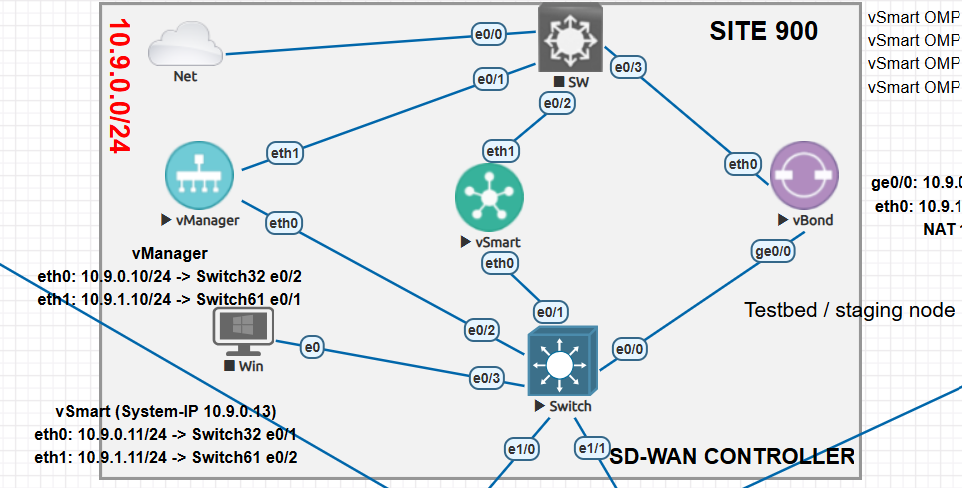
\includegraphics[width=0.75\textwidth]{image/site900.png}
    \caption{Vùng điều khiển SD-WAN (Site 900)}
    \label{fig:site900}
\end{figure}


\begin{table}[H]
    \centering
    \scriptsize
    \caption{System-IP, ASN và TLOC của các vEdge}
    \label{tab:system_ip}
    \begin{tabularx}{\textwidth}{|c|P{2.0cm}|c|P{2.3cm}|c|P{2.6cm}|X|}
        \hline
        \textbf{Site} & \textbf{Thiết bị} & \textbf{Node} & \textbf{System-IP} & \textbf{ASN} & \textbf{TLOC Internet} & \textbf{TLOC MPLS} \\
        \hline
        100 & vEdge1-S100 & 28 & 10.200.100.1 & 65000 & 203.0.113.1/30 & 100.64.100.1/30 \\
        \hline
        100 & vEdge2-S100 & 6 & 10.200.100.2 & 65000 & 203.0.113.5/30 & 100.64.100.5/30 \\
        \hline
        200 & vEdge1-S200 & 29 & 10.200.200.1 & 65010 & -- & 100.64.200.1/30 \\
        \hline
        200 & vEdge2-S200 & 42 & 10.200.200.2 & 65010 & 203.0.113.9/30 & -- \\
        \hline
        300 & vEdge1-S300 & 30 & 10.200.30.1 & 65020 & -- & 100.64.30.1/30 \\
        \hline
        300 & vEdge2-S300 & 40 & 10.200.30.2 & 65020 & 203.0.113.13/30 & -- \\
        \hline
        400 & vEdge1-S400 & 31 & 10.200.40.1 & 65030 & -- & 100.64.40.1/30 \\
        \hline
        400 & vEdge2-S400 & 41 & 10.200.40.2 & 65030 & 203.0.113.17/30 & -- \\
        \hline
        500 & vEdge-S500 & 65 & 10.200.50.1 & 65040 & 203.0.113.21/30 & 100.64.50.1/30 \\
        \hline
    \end{tabularx}
\end{table}

\subsection{Các quyết định thiết kế chính}

\begin{itemize}
    \item \textbf{Control plane SDN đi trong VLAN 99:} kênh OpenFlow dùng chính các uplink sẵn có thay vì mạng điều khiển riêng. Đường VLAN 99 được cắt tỉa thành cây không vòng lặp để controller luôn tới được switch trước khi flow được cài.
    \item \textbf{Core dùng IOL thay vIOS-L2:} image vIOS-L2 bị treo CPU khi có broadcast từ OVS và nạp cấu hình không ổn định; IOL hỗ trợ đầy đủ SVI, VRRP và OSPF.
    \item \textbf{Firewall-as-Core tại chi nhánh:} Brand-FW vừa là gateway vừa cấp DHCP, giảm số thiết bị và giúp chi nhánh vẫn cấp địa chỉ khi WAN gián đoạn.
    \item \textbf{Underlay BGP thay OSPF:} mô phỏng đúng quan hệ khách hàng--nhà cung cấp; vEdge học default route động từ cả hai transport.
    \item \textbf{Site 500 mạng phẳng:} minh họa mô hình chi nhánh nhỏ chi phí thấp, chứng minh việc thêm site mới chỉ cần cấp Site ID, System-IP, chứng thư và cập nhật danh sách site trong chính sách.
\end{itemize}

\subsection{Phương án dự phòng}

Dự phòng được bố trí ở từng tầng để một sự cố đơn lẻ không làm gián đoạn toàn bộ dịch vụ. Bảng~\ref{tab:du_phong} tổng hợp cơ chế dự phòng và các điểm lỗi đơn còn tồn tại trong thiết kế hiện tại.

\begin{table}[H]
    \centering
    \small
    \caption{Cơ chế dự phòng theo từng tầng}
    \label{tab:du_phong}
    \begin{tabularx}{\textwidth}{|P{3.0cm}|X|P{3.6cm}|}
        \hline
        \textbf{Tầng / thành phần} & \textbf{Cơ chế dự phòng} & \textbf{Ghi chú} \\
        \hline
        Gateway Campus chính & VRRP giữa Core-SW1 và Core-SW2 & Máy trạm giữ nguyên gateway .1 \\
        \hline
        Firewall Campus chính & Cặp ASAv active--standby, đồng bộ cấu hình & Kiểm thử failover ở giai đoạn cuối \\
        \hline
        WAN Campus chính & Hai vEdge, mỗi vEdge có cả Internet và MPLS & Dự phòng cả thiết bị và đường truyền \\
        \hline
        WAN chi nhánh 200--400 & Hai vEdge, mỗi vEdge một transport & Mất một vEdge vẫn còn transport kia \\
        \hline
        WAN Site 500 & Một vEdge với hai transport & Chỉ dự phòng đường truyền \\
        \hline
        Đường hầm SD-WAN & BFD phát hiện mất kết nối, AAR chuyển đường theo SLA & Chu kỳ đo ảnh hưởng thời gian chuyển \\
        \hline
        Controller SDN & Một controller Ryu & Điểm lỗi đơn; OVS giữ flow đã cài \\
        \hline
        Controller SD-WAN & Một vManage, một vSmart, một vBond & Data plane vẫn chạy trong thời gian ân hạn \\
        \hline
    \end{tabularx}
\end{table}

\subsection{Luồng lưu lượng điển hình}

Để minh họa cách các thành phần phối hợp, xét một máy trạm VLAN 60 tại Site 200 truy cập Web Server trong DMZ của Campus chính. Gói tin đi qua switch phòng ban và SwitchBrand tới Brand-FW, nơi đóng vai trò gateway và kiểm tra ACL. Brand-FW chuyển gói tới vEdge chi nhánh trong service VPN 1; vEdge tra bảng tuyến học từ OMP, chọn đường hầm IPsec tới vEdge của Site 100 theo chính sách AAR, rồi đóng gói và gửi qua transport tương ứng. Tại Site 100, vEdge giải đóng gói và chuyển gói tới cặp ASAv; firewall chỉ cho phép các dịch vụ đã khai báo đi vào DMZ. Chiều về đi theo đường ngược lại. Trong suốt quá trình, vSmart không nằm trên đường dữ liệu mà chỉ phân phối tuyến và chính sách cho các vEdge.

	\newpage

	\section{TIẾN ĐỘ VÀ KẾT QUẢ GIỮA KỲ}\label{sec:tien_do}

Chương này báo cáo trạng thái từng hạng mục tại mốc \mocbaocao. Mỗi kết quả được xếp vào một trong ba mức: \textbf{Hoàn thành} (có bằng chứng kiểm chứng trên lab), \textbf{Đang thực hiện} (đã có một phần cấu hình hoặc kiểm thử) và \textbf{Chưa bắt đầu}. Nhóm không đưa ra con số hiệu năng khi chưa có phép đo lặp lại.

\subsection{Tổng hợp tiến độ theo hạng mục}

\begingroup
\scriptsize
\setlength{\tabcolsep}{3pt}
\begin{longtable}{|c|P{5.2cm}|P{2.2cm}|P{5.4cm}|}
    \caption{Trạng thái 20 hạng mục tại mốc giữa kỳ}\label{tab:tien_do} \\
    \hline
    \textbf{\#} & \textbf{Hạng mục} & \textbf{Trạng thái} & \textbf{Bằng chứng / ghi chú} \\
    \hline
    \endfirsthead
    \multicolumn{4}{c}{\textit{Bảng~\ref{tab:tien_do} (tiếp theo)}} \\
    \hline
    \textbf{\#} & \textbf{Hạng mục} & \textbf{Trạng thái} & \textbf{Bằng chứng / ghi chú} \\
    \hline
    \endhead
    \hline
    \endfoot
    1 & Khảo sát, xác định phạm vi và mục tiêu & Hoàn thành & Phạm vi 4 site + controller trên EVE-NG \\
    \hline
    2 & Lý thuyết SDN (OpenFlow, Ryu, OVS) & Hoàn thành & Đối chiếu với hành vi thực tế trong lab \\
    \hline
    3 & Lý thuyết SD-WAN (controller, OMP, BFD, TLOC) & Hoàn thành & Tài liệu giải thích tunnel SD-WAN \\
    \hline
    4 & Thiết kế kiến trúc 4 campus & Hoàn thành & Tài liệu thiết kế, Chương~\ref{sec:thiet_ke} \\
    \hline
    5 & Quy hoạch IP, VLAN, DHCP, ASN & Hoàn thành & Bảng~\ref{tab:vlan_campus}--\ref{tab:system_ip} \\
    \hline
    6 & Topology EVE-NG và quy trình đồng bộ cấu hình & Hoàn thành & 67 node, 100 network, 47 cấu hình nhúng; công cụ kiểm tra \texttt{.unl} báo ĐẠT \\
    \hline
    7 & Core/Dist/Access, VLAN, trunk, VRRP, OSPF & Hoàn thành & Firewall học đủ tuyến \texttt{10.1.x} qua OSPF \\
    \hline
    8 & Firewall ASAv HA và quản trị ASDM & Hoàn thành & \texttt{show failover}: Primary Active, Secondary Standby Ready \\
    \hline
    9 & DHCP-Server và cấp phát end-to-end & Hoàn thành & 8/8 VPC Site 100 nhận địa chỉ qua relay (20/09) \\
    \hline
    10 & Ryu + kết nối 6 OVS & Hoàn thành & 6/6 OVS kết nối controller ổn định \\
    \hline
    11 & Ứng dụng L2 SDN (học MAC theo VLAN, ACL) & Hoàn thành & DHCP và ping liên VLAN qua OVS thành công \\
    \hline
    12 & Ba controller SD-WAN và PKI & Hoàn thành & vManage, vSmart, vBond hoạt động, CA nội bộ \\
    \hline
    13 & Onboard 8 vEdge, BFD và control connection & Hoàn thành & 8/8 vEdge lên controller; BFD 56/56 up (23/09) \\
    \hline
    14 & Định tuyến liên site và chính sách SD-WAN & Hoàn thành & Service VPN 1, OMP; SLA, AAR, data policy, control policy \\
    \hline
    15 & Chi nhánh 200/300/400: Brand-FW, switch, VPC & Hoàn thành & DHCP cục bộ, router-on-a-stick, ACL \texttt{SDWAN\_IN} \\
    \hline
    16 & vEdge chi nhánh join fabric, 2 hướng SP & Hoàn thành & 6 vEdge chi nhánh trong fabric \\
    \hline
    16b & Chi nhánh mới Site 500 (mạng phẳng) & Đang thực hiện & Đã đấu nối Internet/MPLS, cấu hình vEdge và cài chứng thư (01/10); còn whitelist controller, cấu hình SP, policy \\
    \hline
    17 & Dịch vụ Web/Mail/DNS/Syslog & Hoàn thành phần chính & DNS, HTTPS, gửi/nhận mail từ chi nhánh qua SD-WAN \\
    \hline
    18 & Kiểm thử tích hợp end-to-end & Đang thực hiện & Đã có DHCP, ping liên site, BFD, AAR; còn failover FW HA, mất controller \\
    \hline
    19 & Báo cáo cuối kỳ & Đang thực hiện & Bản nháp các chương; báo cáo giữa kỳ này \\
    \hline
    20 & Slide và demo trực tiếp & Chưa bắt đầu & Dự kiến 11/2026 \\
\end{longtable}
\endgroup

Trong 21 hạng mục (gồm hạng mục 16b mới bổ sung), 16 hạng mục đã hoàn thành, 1 hạng mục hoàn thành phần chính (dịch vụ), 3 hạng mục đang thực hiện và 1 hạng mục chưa bắt đầu. Toàn bộ phần thiết kế và phần triển khai cốt lõi đã xong; khối lượng còn lại tập trung vào kiểm thử, mở rộng Site 500 và tài liệu.

\subsection{Kết quả đã đạt được}

\subsubsection{Hạ tầng Campus chính}

Core-SW1/2 cung cấp gateway VRRP cho các VLAN 10/20/30/40/90 và trao đổi tuyến OSPF với firewall active. Cặp ASAv hoạt động active--standby, cấu hình tự đồng bộ sang unit dự phòng; PC quản trị truy cập ASDM qua VLAN 99. DHCP Server (Windows Server 2012 R2) có bốn scope cho bốn VLAN người dùng; 8/8 máy trạm Site 100 nhận đúng địa chỉ qua DHCP relay trên Core.

\subsubsection{SDN}

Bộ điều khiển Ryu tại \texttt{10.1.99.10} quản lý sáu OVS (Dist-SW1/2, Access-SW1--4) bằng OpenFlow 1.3. Các phép thử độ bền đã thực hiện:

\begin{itemize}
    \item Khởi động lại Ryu: cả 6 switch kết nối lại trong khoảng 15 giây.
    \item Khởi động lại từng Access Switch: switch quay lại trong khoảng 2,5 phút.
    \item Tắt hẳn Dist-SW1: 5 switch còn lại giữ kết nối với controller; bật lại thì hệ thống tự phục hồi 6/6 trong khoảng 2 phút.
\end{itemize}

Ngoài Ryu, nhóm cài thêm ONOS 2.7 chạy song song làm giao diện giám sát: ONOS nhận đủ 6 thiết bị và các liên kết giữa chúng, trong khi Ryu vẫn đảm nhận chuyển tiếp.

\subsubsection{SD-WAN}

Fabric gồm ba controller và tám vEdge thuộc Site 100--400. Kết quả kiểm chứng ngày 23/09/2026:

\begin{itemize}
    \item 8/8 vEdge có control connection tới vBond, vSmart, vManage.
    \item 56/56 phiên BFD up, gồm cả các đường hầm chéo màu Internet--MPLS.
    \item Service VPN 1 trên tám vEdge; OMP quảng bá subnet của bốn site; máy trạm các site ping thông nhau.
    \item Chính sách tập trung trên vSmart: Application-Aware Routing cho ICMP, thoại, web và mail theo hai lớp SLA là \texttt{SLA\_REALTIME} và \texttt{SLA\_BUSINESS}; data policy chặn Telnet/SSH từ chi nhánh vào Server Farm và DMZ; control policy ưu tiên vEdge1 của Site 100.
\end{itemize}

Ngày 26/09/2026, nhóm thử AAR bằng cách tạo trễ nhân tạo 1000~ms trên một đường WAN của Site 100. Lưu lượng ICMP từ Site 200 đã chuyển khỏi đường hầm bị trễ. Do chu kỳ đo BFD được đặt dài (\texttt{poll-interval} 120~s), thời gian chuyển đường thực tế là vài phút; đây là kết quả của một lần thử, chưa phải số liệu đo lặp.

\subsubsection{Dịch vụ qua SD-WAN}

Từ máy trạm Linux tại Site 200, nhóm kiểm tra phân giải DNS bản ghi \texttt{mail}/\texttt{MX}, truy cập HTTPS tới Web Server trong DMZ (máy chủ thấy địa chỉ thật của máy trạm, không bị NAT) và gửi/nhận thư qua cổng 587/IMAP. Firewall Site 100 chỉ mở đúng các dịch vụ cần thiết từ SD-WAN vào DMZ; các cổng khác bị chặn và ghi log.

\subsection{Vấn đề kỹ thuật đã gặp và cách xử lý}

Bảng~\ref{tab:van_de} tổng hợp các sự cố tiêu biểu. Mỗi sự cố được xác định nguyên nhân bằng chẩn đoán theo lớp trước khi sửa.

\begingroup
\scriptsize
\setlength{\tabcolsep}{3pt}
\begin{longtable}{|P{3.3cm}|P{4.7cm}|P{4.8cm}|}
    \caption{Một số vấn đề kỹ thuật và cách xử lý}\label{tab:van_de} \\
    \hline
    \textbf{Hiện tượng} & \textbf{Nguyên nhân} & \textbf{Cách xử lý} \\
    \hline
    \endfirsthead
    \multicolumn{3}{c}{\textit{Bảng~\ref{tab:van_de} (tiếp theo)}} \\
    \hline
    \textbf{Hiện tượng} & \textbf{Nguyên nhân} & \textbf{Cách xử lý} \\
    \hline
    \endhead
    \hline
    \endfoot
    Máy trạm Site 100 không nhận DHCP qua OVS & Luật table-miss không gửi gói lên controller; ứng dụng đọc VLAN sai trường (\texttt{dl\_vlan} của OpenFlow 1.0 thay vì \texttt{vlan\_vid}) & Sửa luật table-miss và cách so khớp VLAN trong ứng dụng Ryu \\
    \hline
    Bão broadcast, switch mất kết nối controller & VLAN 99 có vòng lặp khi tắt STP trên OVS & Cắt tỉa VLAN 99 thành cây không vòng lặp, cài flow bootstrap cho VLAN 99 \\
    \hline
    vEdge kẹt ở trạng thái \textit{connect} & Chứng thư có trường O khác ``Cisco Systems'' nên vBond/vSmart từ chối & Ký lại chứng thư với subject đúng chuẩn \\
    \hline
    vEdge rơi khỏi fabric sau khi controller khởi động lại & Danh sách thiết bị được phép trên vBond chỉ lưu trong bộ nhớ & Đẩy lại danh sách từ vManage; đưa bước kiểm tra whitelist vào quy trình sau mỗi lần khởi động lại controller \\
    \hline
    Màu \texttt{biz-internet} không có đường tới controller & Route /24 qua MPLS che route /16 qua Internet (longest-prefix) & Thêm route /24 cùng độ dài qua cả hai transport \\
    \hline
    Tunnel Internet--MPLS down hàng loạt & Khai sai màu TLOC trên vEdge2 chi nhánh & Sửa màu đúng với loại đường truyền \\
    \hline
    BFD chéo màu Site 100 down & Mỗi TLOC chỉ có đường tới transport còn lại qua một cổng & Thêm default route cho từng transport trong VPN 0 \\
    \hline
    Cổng MPLS của vEdge2-S100 không nhận gói & Card mạng ảo bị treo phía nhận & \texttt{shutdown}/\texttt{no shutdown} cổng; BGP và TLOC lên lại \\
\end{longtable}
\endgroup

\subsection{Đánh giá giữa kỳ}

Tiến độ thực tế bám sát kế hoạch: giai đoạn khảo sát, thiết kế và triển khai đã hoàn thành đúng hoặc sớm hơn mốc dự kiến (hạng mục 16 có hạn 15/10/2026). Điểm mạnh của giai đoạn vừa qua là mọi kết quả đều có bằng chứng từ thiết bị và các sự cố đều được ghi nhận nguyên nhân gốc, tạo thành tài liệu vận hành có giá trị.

Các hạn chế hiện tại:

\begin{itemize}
    \item Chưa có bộ đo hiệu năng lặp lại (thông lượng, độ trễ, thời gian hội tụ); các con số hiện có là kết quả của từng lần thử.
    \item SDN chỉ có một controller Ryu, là điểm lỗi đơn của mặt phẳng điều khiển.
    \item Đợt rớt kết nối đồng loạt của các vEdge trong đêm 22--23/09/2026 đã tự hết nhưng chưa xác định được nguyên nhân.
    \item Một số bước triển khai vẫn làm thủ công (Windows, OVS, controller SD-WAN), phụ thuộc vào việc tuân thủ đúng quy trình.
\end{itemize}

	\newpage

	\section{KẾ HOẠCH GIAI ĐOẠN CUỐI VÀ KẾT LUẬN}\label{sec:ke_hoach}

\subsection{Kế hoạch công việc còn lại}

Bảng~\ref{tab:ke_hoach_cuoi} liệt kê các công việc từ mốc giữa kỳ đến ngày bảo vệ dự kiến (cuối tháng 11/2026).

\begin{table}[H]
    \centering
    \small
    \caption{Kế hoạch giai đoạn cuối}
    \label{tab:ke_hoach_cuoi}
    \begin{tabularx}{\textwidth}{|c|X|P{3.0cm}|P{3.6cm}|}
        \hline
        \textbf{\#} & \textbf{Công việc} & \textbf{Thời gian} & \textbf{Kết quả cần đạt} \\
        \hline
        1 & Hoàn thiện Site 500: whitelist trên 3 controller, cấu hình BGP phía nhà cung cấp, thêm site vào chính sách vSmart, nối switch và máy trạm & 02/10--10/10 & vEdge-S500 lên fabric; máy trạm nhận DHCP và ping được các site \\
        \hline
        2 & Kiểm thử failover: firewall HA, mất một transport, mất một vEdge tại chi nhánh & 10/10--25/10 & Biên bản kiểm thử có điều kiện, kết quả và thời gian hội tụ \\
        \hline
        3 & Kiểm thử SDN khi mất controller và khi có lưu lượng mới & 15/10--30/10 & Mô tả hành vi OVS ở chế độ \texttt{secure} khi mất Ryu \\
        \hline
        4 & Đo lặp lại độ trễ, mất gói và thời gian chuyển đường AAR & 20/10--05/11 & Bảng số liệu nhiều lần đo, có giá trị trung bình \\
        \hline
        5 & Tìm nguyên nhân đợt rớt kết nối vEdge 22--23/09 nếu tái diễn & Theo dõi liên tục & Kết luận nguyên nhân hoặc ghi nhận không tái diễn \\
        \hline
        6 & Hoàn thiện báo cáo cuối kỳ & 01/11--20/11 & Báo cáo đầy đủ 5 chương, cập nhật số liệu kiểm thử \\
        \hline
        7 & Slide và kịch bản demo trên lab & 10/11--20/11 & Slide; kịch bản demo đã chạy thử \\
        \hline
    \end{tabularx}
\end{table}

\subsection{Rủi ro và biện pháp}

\begin{itemize}
    \item \textbf{Tài nguyên máy chủ EVE-NG:} lab 67 node cần nhiều RAM/CPU; khi chạy đồng thời dễ gây chậm hoặc treo node. Biện pháp: bật theo thứ tự đã kiểm chứng, chỉ chạy các site cần cho từng phép thử.
    \item \textbf{Mất trạng thái khi wipe node:} vEdge mất chứng thư, Windows/OVS mất cấu hình tay. Biện pháp: không wipe các node này; lưu cấu hình và quy trình phục hồi trong kho mã nguồn.
    \item \textbf{Whitelist controller mất sau khởi động lại:} vEdge rơi khỏi fabric mà không có cảnh báo rõ ràng. Biện pháp: kiểm tra whitelist sau mỗi lần khởi động lại controller và đẩy lại từ vManage.
    \item \textbf{Thời gian:} khối lượng kiểm thử và viết báo cáo dồn vào tháng 11. Biện pháp: thực hiện kiểm thử song song với viết báo cáo, ghi kết quả ngay sau mỗi phép thử.
\end{itemize}

\subsection{Kết luận giữa kỳ}

Đến mốc giữa kỳ, nhóm đã hoàn thành phần thiết kế và phần lớn khối lượng triển khai của đề tài. Mô hình trên EVE-NG đã thể hiện được các mục tiêu chính: Campus chính phân tầng với gateway dự phòng và firewall HA, SDN điều khiển sáu switch OVS bằng Ryu, fabric SD-WAN kết nối bốn site qua hai transport với chính sách chọn đường theo SLA, cùng các dịch vụ mạng truy cập được từ chi nhánh. Việc bổ sung Site 500 theo mô hình mạng phẳng cho thấy kiến trúc có thể mở rộng bằng quy trình rõ ràng.

Nửa còn lại của dự án tập trung vào kiểm thử có số liệu, hoàn thiện chi nhánh mới và tài liệu. Nhóm đánh giá dự án đang đúng tiến độ và đủ điều kiện để hoàn thành các mục tiêu đã đề ra trước ngày bảo vệ.

	\newpage

	% --- PHẦN CUỐI CỦA BÁO CÁO ---
	\nocite{*}
	\bibliography{tailieuthamkhao}

\end{document}
